% --------------------------------------------------------------
% This is all preamble stuff that you don't have to worry about.
% Head down to where it says "Start here"
% --------------------------------------------------------------
 
\documentclass[12pt]{article}
 
\usepackage[margin=1in]{geometry} 
\usepackage{amsmath,amsthm,amssymb}
 \usepackage{algorithmic}
 \usepackage{graphicx}
\newcommand{\N}{\mathbb{N}}
\newcommand{\Z}{\mathbb{Z}}
 
\newenvironment{theorem}[2][Theorem]{\begin{trivlist}
\item[\hskip \labelsep {\bfseries #1}\hskip \labelsep {\bfseries #2.}]}{\end{trivlist}}
\newenvironment{lemma}[2][Lemma]{\begin{trivlist}
\item[\hskip \labelsep {\bfseries #1}\hskip \labelsep {\bfseries #2.}]}{\end{trivlist}}
\newenvironment{exercise}[2][Exercise]{\begin{trivlist}
\item[\hskip \labelsep {\bfseries #1}\hskip \labelsep {\bfseries #2.}]}{\end{trivlist}}
\newenvironment{reflection}[2][Reflection]{\begin{trivlist}
\item[\hskip \labelsep {\bfseries #1}\hskip \labelsep {\bfseries #2.}]}{\end{trivlist}}
\newenvironment{proposition}[2][Proposition]{\begin{trivlist}
\item[\hskip \labelsep {\bfseries #1}\hskip \labelsep {\bfseries #2.}]}{\end{trivlist}}
\newenvironment{corollary}[2][Corollary]{\begin{trivlist}                      
\item[\hskip \labelsep {\bfseries #1}\hskip \labelsep {\bfseries #2.}]}{\end{trivlist}}
\newenvironment{definition}[2][definition]{\begin{trivlist}                      
\item[\hskip \labelsep {\bfseries #1}\hskip \labelsep {\bfseries #2.}]}{\end{trivlist}}
 
\begin{document}
 
% --------------------------------------------------------------
%                         Start here
% --------------------------------------------------------------
 
%\renewcommand{\qedsymbol}{\filledbox}
 
\title{Homework \#9}%replace X with the appropriate number
\author{Tanner Hammond\\ %replace with your name
CPSC 395 - Analysis of Algorithms
\\ Due: Monday, 19} %if necessary, replace with your course title
\date{}
\maketitle

\begin{enumerate}
\item Exercise 16.1-1 \\
Give a dynamic-programming algorithm for the activity-selection problem, based on recurrence (16.2). Have your algorithm compute the sizes c[i,j] as defined above and also produce the maximum-size subset of mutually compatible activities. Assume that the inputs have been sorted as in equation (16.1). Compare the running time of your solution to the running time of GREEDY-ACTIVITY-SELECTOR.

Recurrence 16.2: c[i,j] = $\{^{0 \qquad if S_{ij} = \O}_{max_{a_k \in S_{ij}} \{c[i,k] + c[k,j] + 1\}\quad if S_{ij} \neq \O}$. The inputs are the arrays s and f which are the start and finish times and n is the number of activities.

DYNAMIC-ACTIVITY-SELECTION(s,f,n)
\begin{algorithmic}
\STATE c[i,j]
\FOR{i = 1 to n}
\FOR{j = 2 to n}
\STATE c[i,j] = 0
\FOR{k = i+1 to j-1}
\IF{s[k] $\geq$ f[i]}
\STATE c[i,j] = c[i,k] + c[k,j] + 1
\ENDIF
\ENDFOR
\ENDFOR
\ENDFOR
\STATE return c
\end{algorithmic}


GREEDY-ACTIVITY-SELECTOR(s,f)
\begin{algorithmic}
\STATE n = s.length
\STATE A = \{$a_1$\}
\STATE k = 1
\FOR {m = 2 to n}
\IF {s[m] $\geq$ f[k]}
\STATE A = A $\bigcup$ \{$a_m$\}
\STATE k = m
\ENDIF
\ENDFOR
\STATE return A
\end{algorithmic}

Now to compare the run time of the dynamic programming algorithm and the greedy algorithm. The greedy algorithm has a run time of $\Theta(n)$. The run time for the dynamic is $\Theta(n^3)$.

\item Exercise 16.1-3 \\
Not just any greedy approach to the activity-selection problem produces a maximum-size set of mutually compatible activities. Give an example to show that the approach of selecting the activity of least duration from among those that are compatible with previously selected activities does not work. Do the same for the approaches of always selecting the compatible activity that overlaps the fewest other remaining activities and always selecting the compatible remaining activity with the earliest start time. \\

So the approach of selecting activities by the least duration doesn't work because while an activity may have the least duration, it could conflict with the times of the other activities and will not return an optimal solution. An example would be if there is 3 activities; Activity 1 with start and finish (2,6), Activity 2 with start,finish (5,7), and Activity 3 with start,finish (6,11). Activity 1 has a duration of  4, 2 a duration of 2, and 3 a duration of 5. The first activity to be picked will be Activity 2 since it has the least duration, but it will be the only one in the subset since the other classes are compatible. But as can be seen, the solution of Activity 1 and 3 exists and is more optimal. \\

For the approach of selecting by the least amount of overlaps:
\begin{center}
 \begin{tabular}{||c c c c||} 
 \hline
 Activity i & Starting Time & Finishing Time & Number of Overlaps\\ [0.5ex] 
 \hline
 1 & 4 & 6 & 2 \\ 
 \hline
 2 & 2 & 4 & 3 \\
 \hline
 3 & 1 & 3 & 2 \\
 \hline
 4 & 3 & 5 & 3 \\
 \hline
 5 & 6 & 8 & 3 \\
 \hline
 6 & 6 & 8 & 3  \\ 
 \hline
 7 & 7 & 9 & 2  \\ 
 \hline
 8 & 2 & 4 & 3  \\
 \hline
 9 & 5 & 7 & 2  \\
 \hline
\end{tabular}
\end{center}

This approach would give the solution of \{1,3,7\}, but another solution that is better would be \{3,4,7,9\}. 

The last approach for selecting activities by the earliest start times will not always be the most efficient either. In the case if there were these activities:

\begin{center}
 \begin{tabular}{||c c c||} 
 \hline
 Activity i & Starting Time & Finishing Time\\ [0.5ex] 
 \hline
 1 & 1 & 6\\ 
 \hline
 2 & 2 & 4\\
 \hline
 3 & 4 & 7\\
 \hline
 4 & 6 & 8\\
 \hline
 5 & 7 & 10 \\
 \hline
\end{tabular}
\end{center}

The solution it would give would be \{1,4\}, but the more optimal solution would be \{2,4,5\}. So all of these approaches will work, but they won't always give the best solutions.

\item Exercise 16.2-5 \\ 
Describe an efficient algorithm that, given a set $\{x_1, x_2, ... , x_n\}$ of points on the real line, determines the smallest set of unit-length closed intervals that contains all of the given points. Argue that your algorithm is correct. \\

An efficient algorithm will be a greedy algorithm. First you would want to sort the set such that the first element is the first point on the line and the last in the set is the last point on the line. We're trying to find the smallest set of closed intervals so we will have the set S which contains the intervals. The first interval will be [$x_1$, $x_1$ + 1]. This will be added to the set S and the points not within the interval will be removed from the set of points. The next intervals will be [$x_i$, $x_i$ + 1] and the process will be repeated until the set of points is empty and the set S will be returned. 

\item Exercise 16.3-3 \\
What is an optimal Huffman code for the following set of frequencies, based on the first 8 Fibonacci numbers?  a:1 b:1 c:2 d:3 e:5 f:8 g:13 h:21
The tree for the set of frequencies:\\
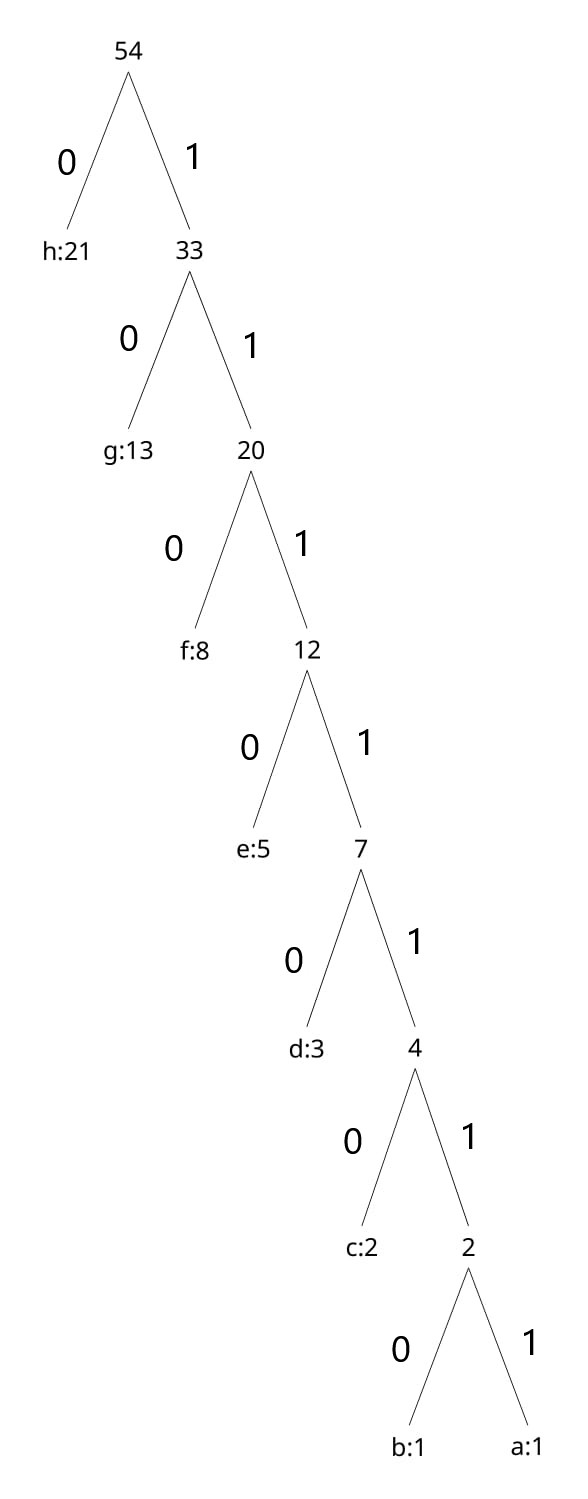
\includegraphics[scale=.45]{54-2.jpg}\\
The Huffman code for this is:
\begin{algorithmic}
\STATE h:0
\STATE g:10
\STATE f:110
\STATE e:1110
\STATE d:11110
\STATE c:111110
\STATE b:1111110
\STATE a:1111111
\end{algorithmic}
Can you generalize your answer to find the optimal code when the frequencies are the first n Fibonacci numbers?\\
With the Fibonacci sequence, $F_{n+2}$ = $F_{n+1}$ + $F_n$. $\sum_{i=0}^{n-1} F_i + 1 + F_n$ . $\sum_{i=0}^n F_i + 1$. So the generalization of the first n numbers is $\sum_{i=0}^n F_i + 1$
\end{enumerate}

% --------------------------------------------------------------
%     You don't have to mess with anything below this line.
% --------------------------------------------------------------
 
\end{document}